% !TEX root = ../main.tex
\section{Experiment}
\label{11::experiment}
    The Thomas Jefferson National Accelerator Facility is a High Energy Physics (HEP) laboratory located in Newport News, Virginia, USA.
    For simplicity and to follow convention, the laboratory will be called JLab hereafter.
    At the site, there is a recirculating linear electron accelerator named the Continuous Electron Beam Accelerator Facility (CEBAF).
    This accelerator is capable of delivering a 12 GeV electron beam to four experimental Halls simultaneously: Halls A, B, C, and D.

    Different physics topics are studied in each of these halls.
    This thesis aims to provide a preparatory study for the RG-E experiment, which will take place in Hall B, where the CEBAF Large Acceptance Spectrometer for operation at 12 GeV (CLAS12) is located.

    The first section provides a brief description of CEBAF at JLab.
    The second section then provides detailed information about CLAS12, including its central detector, forward detector, and offline event reconstruction.
    The third and final section discusses the RG-E experiment to be performed.

    % !TEX root = ../main.tex
\subsection{CEBAF}
\label{11.100::cebaf}
    \begin{figure}[b!]
        \centering\frame{
        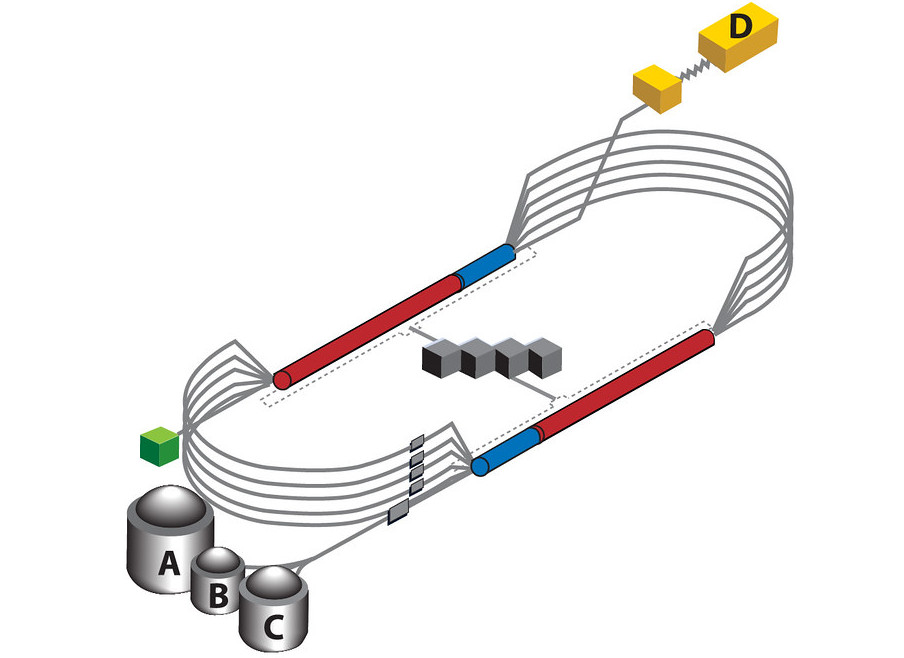
\includegraphics[width=\textwidth]{100cebaf_diagram.jpg}}
        \caption[CEBAF.]{Simplified representation of CEBAF.
        Source: \hyperlink{jlab.org/}{jlab.org}.}
        \label{fig::11.100::cebaf}
    \end{figure}

    CEBAF consists of a pair of 1.4-km-long antiparallel superconducting radio-frequency (RF) linear accelerators (linacs) constructed 8 meters below the surface.
    The two accelerators are connected by two 180-degree arcs, each with a radius of 80 meters \cite{leemann2001}.
    A schematic diagram illustrating the design of CEBAF is provided in Figure \ref{fig::11.100::cebaf}.

    The recirculating arcs are composed of five separate beamline sections, allowing the beam to traverse each linac up to five times.
    Within each linac, the energy gain of the beam ranges from 0.8 GeV to 1.2 GeV, resulting in a final beam energy of approximately 12 GeV.
    CEBAF is specifically designed for high-energy electron beam experiments aimed at studying the structure of mesons, nucleons, and nuclei \cite{rode2010}.

    % !TEX root = ../main.tex
\subsection{CLAS12}
\label{ssec::clas12}
    \begin{figure}[b!]
        \centering\frame{
        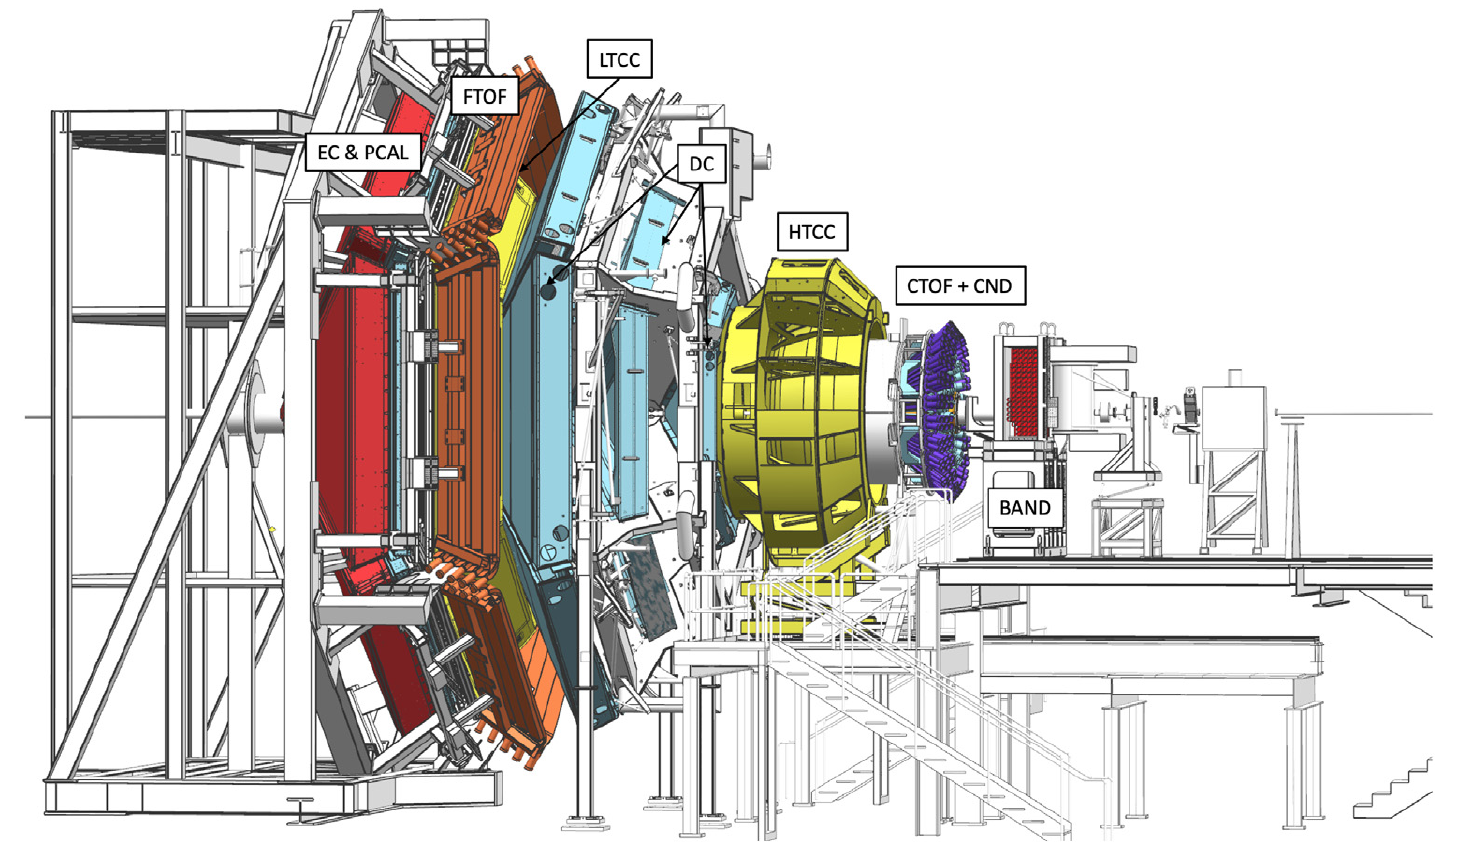
\includegraphics[width=\textwidth]{200clas12_diagram.png}}
        \caption[CLAS12.]{The CLAS12 detector in the Hall B beamline.
        The electron beam enters from the right and impinges on the target located in the center of the solenoid magnet shown at the right (upstream) end of CLAS12.
        The FD consists of the High Threshold Cherenkov Counter (HTCC) (yellow), the torus magnet (grey), the DC tracking system (light blue), and another set of Cherenkov counters (hidden), time-of-flight scintillation counters (brown), and Electromagnetic Calorimeters (ECs) (red).
        Between the HTCC and the torus, the Forward Tagger (FT) is installed.
        The CD consists of the Silicon Vertex Tracker (SVT) (hidden), which is surrounded by a Barrel Micromesh Tracker (BMT) (hidden), the Central Time-of-Flight (FTOF) system, and the Central Neutron Detector (CND) (blue).
        At the upstream end, a Back Angle Neutron Detector (BAND) (red) is installed.
        Source: \hyperlink{https://www.jlab.org/physics/hall-b/clas12}{CLAS12 wiki}.}
        \label{fig::clas12_diagram}
    \end{figure}

    The main detector in Hall B is CLAS12, used to study electro-induced nuclear and hadronic reactions \cite{burkert2020}.
    The spectrometer provides efficient detection of charged and neutral particles over a large fraction of the full solid angle.

    CLAS12 is based on two superconducting magnets: a solenoid magnet and a 5 T torus magnet.
    The detector is divided into two parts: the Forward Detector (FD) and the Central Detector (CD).
    The FD, aided by the torus magnet, covers the forward polar range from $5\degree$ up to $35\degree$, while the CD, aided by the solenoid magnet, covers the polar angles from $35\degree$ to $125\degree$.
    Both detectors have full azimuthal coverage.

    Trajectory reconstruction is performed using Drift Chambers (DC) in the forward direction, achieving a momentum resolution of less than $1\%$.
    In the central detector, trajectory reconstruction is done using a vertex tracker, resulting in a momentum resolution of less than $3\%$.
    Particle identification relies on Cherenkov counters, time-of-flight scintillators, and electromagnetic calorimeters \cite{burkert2020}.
    Fast triggering and high data-acquisition rates enable operation at a luminosity of $10^{35} \text{ cm}^{-2}\text{ s}^{-1}$ \cite{burkert2020}.

    A diagram of CLAS12 showing the position of each detector component is provided in Figure \ref{fig::clas12_diagram}.

    % !TEX root = ../main.tex
\subsubsection{Forward Detector}
\label{sssec::forward_detector}
    % The Forward Detector (FD) is an essential component of the CLAS12 spectrometer designed to detect particles scattered at small polar angles in the forward direction.
    % It consists of several subdetectors that play crucial roles in particle identification, tracking, and timing measurements.
    %
    % Based on its polar coverage, the FD can be divided into two: the Forward Tagger (FT) and the FD proper.
    % The former detects particles with a polar angle between $2.5\degree$ and $4.5\degree$.
    % The latter detects those with a polar angle between $5\degree$ and $35\degree$.
    % A detailed description of each subdetector systems is provided in the following paragraphs.
    %
    % The Forwards Micromegas Tracker (FMT) is part of the FD, but is not included in this list.
    % The detectors is explored in detail in Section \ref{ssec::forwardsmicromegastracker}.

    % !TEX root = ../main.tex
\paragraph{High Threshold Cherenkov Counter (HTCC)}
    \begin{wrapfigure}{l}{0.50\textwidth}
        \centering\frame{
        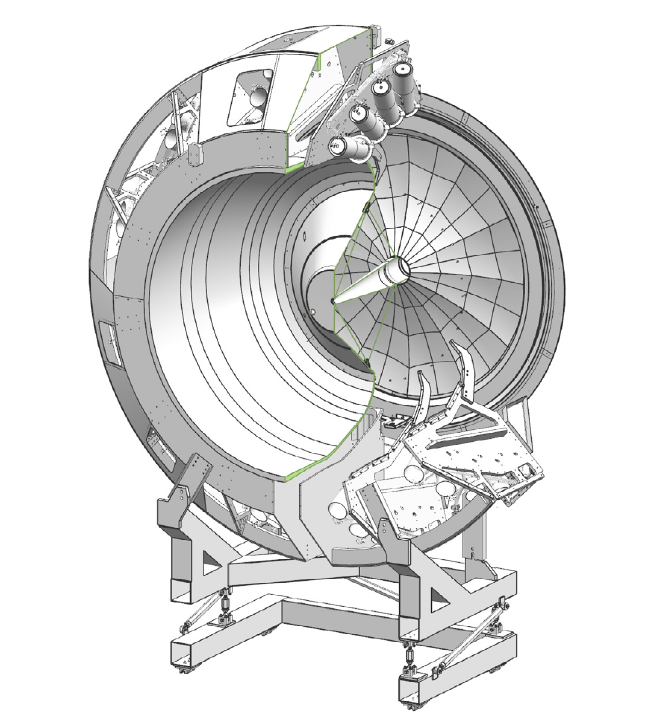
\includegraphics[width=\linewidth]{211htcc.png}}
        \caption[HTCC]{Render of the High Threshold Cherenkov Counter.
        The container spans a diameter of about 4.5 m. The mirror is seen at the downstream end to the right.
        The PMTs are mounted in 12 sectors and in groups of 4 at the outer perimeter of the container.
        Light collection uses additional Winston cones and 5-in PMTs with quartz windows.
        Source: \hyperlink{jlab.org/physics/hall-b/clas12}{CLAS12 wiki}.}
        \label{fig::htcc}
    \end{wrapfigure}

    The HTCC is specifically designed to separate electrons and positrons with momenta below 4.9 GeV from other charged particles.
    It achieves this through its capability for electron/positron identification, which provides high rejection of charged pions and low background noise.
    This is crucial for reliably identifying scattered electrons in an environment with a dense electromagnetic background.

    The HTCC is positioned downstream of the target and is fitted in between magnets, upstream of the forward tracking detectors.
    It ensures full azimuthal coverage, meaning it can detect particles emitted from any direction around its circumference.
    In terms of the polar angle, it spans from $5\degree$ to $35\degree$, covering a specific range of particle emission angles.
    Importantly, it has no blind areas in its complete solid angle coverage, meaning there are no regions where particles cannot be detected.

    Operating in dry CO2 gas at 1 atm pressure, the HTCC consists of a multi-focal mirror composed of 48 elliptical mirror facets.
    This mirror design enables the focusing of Cherenkov light produced by charged particles passing through the detector.
    The focused light is then detected by 48 Photomultiplier Tubes (PMTs), with each PMT featuring a quartz window of 125 mm in diameter.

    The PMTs are positioned within a magnetic field of up to $3.5\cdot 10^{-3}$ T, which is oriented along the axes of the phototubes.
    To minimize the impact of the magnetic field on the PMTs, they are surrounded along their lengths by a multi-layer magnetic shield.
    This shield includes active compensation coils, which further help in shielding the PMTs from the effects of the magnetic field.

    To minimize the effects of multiple scattering and its impact on the momentum analysis of charged tracks in the torus field, the HTCC mirror system is constructed using a backing structure made of low-density composite material.
    This choice of material helps to reduce the scattering of particles passing through the HTCC, thereby improving the accuracy of momentum measurements.

    Since the HTCC is located in front of the momentum analyzing torus magnet, it is important to minimize the presence of materials in the path of charged particles, except for the radiator gas.
    This is done to prevent interactions and disturbances that could affect the accuracy of momentum analysis.
    The HTCC is designed with this consideration in mind.

    In the HTCC, the density of solid material encountered by charged particles passing through its volume is approximately $135~\text{mg/cm}^2$.
    This low-density configuration ensures that the material contribution to multiple scattering is minimised, allowing for more precise momentum measurements of charged tracks.

    The HTCC also serves the purpose of generating a fast signal that can be used as a trigger for scattered electrons.
    This signal is utilised to identify and select scattered electrons for further analysis.

    In conjunction with the energy deposited in the electromagnetic calorimeters, the HTCC plays a role in the identification of electrons with specific energies.
    By combining the information from the HTCC and the electromagnetic calorimeters, the experiment can accurately identify electrons of interest based on their energy deposition patterns.

    A visual representation of the HTCC can be seen in Figure \ref{fig::htcc}, which provides a cut view of the detector and its components.

    Overall, the HTCC plays a crucial role in electron/positron identification by using a multi-focal mirror, PMTs, and a magnetic field setup.
    These components work together to ensure efficient detection and separation of electrons and positrons from other charged particles in a high-energy physics experiment environment.

    % !TEX root = ../main.tex
\paragraph{Drift Chambers (DC)}
    The forward tracking system in the experiment consists of three independent drift chambers in each of the six sectors of the torus magnet.
    These drift chambers serve as the primary tracking detectors and are supported by the six coils of the torus magnet.

    Each sector of the torus magnet contains a total of 36 layers in the drift chambers, with each layer having 112 sense wires.
    The sense wires are arranged in three regions, with each region comprising twelve layers.
    This configuration results in a total of 112 x 36 sense wires per sector.

    \begin{wrapfigure}{r}{0.50\textwidth}
        \frame{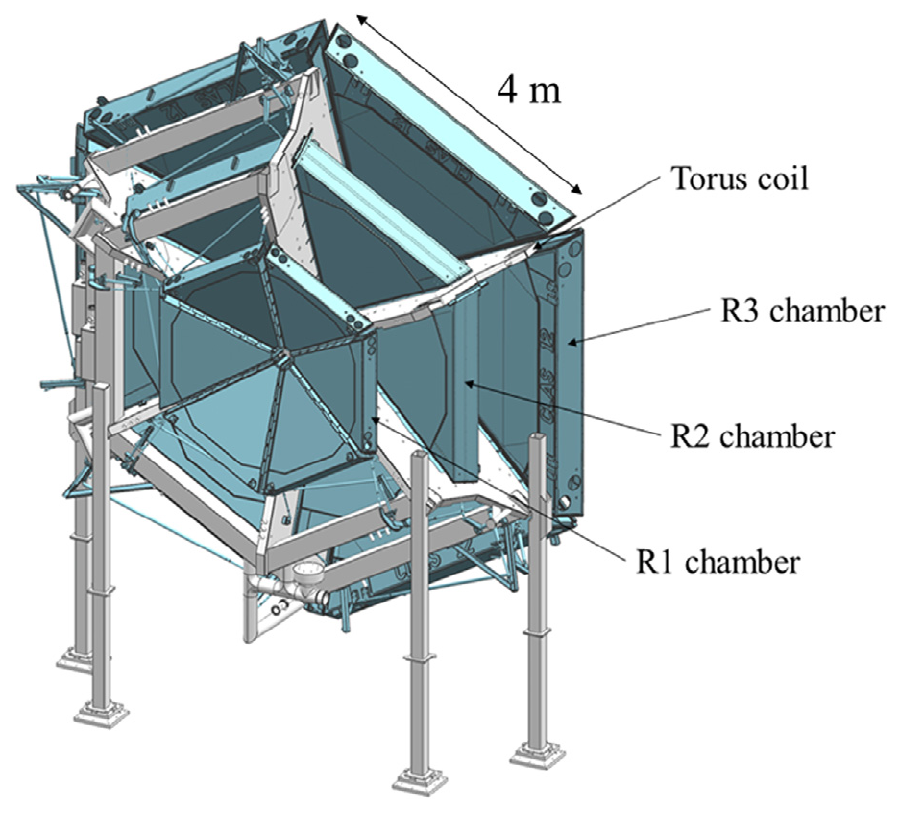
\includegraphics[width=\linewidth]{212dc.png}}
        \caption[DC]
        {Drift Chambers (DC) render.
        Each of the DC regions are denoted as R1, R2, and R3 in the figure.}
        \floatfoot{Source: \href{https://jlab.org/physics/hall-b/clas12}{CLAS12 wiki}.}
        \label{fig::11.212::dc}
    \end{wrapfigure}

    The arrangement of the drift chambers around the torus coil can be visualised in Figure \ref{fig::11.212::dc}.
    The figure shows the positioning of the three regions of the drift chambers in each sector of the torus magnet.

    In terms of location, the first region of the drift chambers is situated at the entrance to the torus magnetic field region.
    The second region is positioned inside the magnet, where the magnetic field is close to its maximum strength.
    Finally, the third region is located downstream of the torus magnet, in a low magnetic field space.

    This arrangement of the drift chambers around the torus magnet provides independent and redundant tracking capabilities in each of the six torus sectors.
    It allows for precise reconstruction of charged particle trajectories and momentum measurements in the experiment.

    Each of the three regions in the drift chambers consists of six "superlayers," where each superlayer comprises two layers.
    The wires in one layer are strung at a stereo angle of $+6\degree$ relative to the sector midplane, while the wires in the other layer are strung at a stereo angle of $-6\degree$.
    This stereo configuration provides excellent resolution in the polar angle ($\Delta\theta < 2 ~\text{mrad}$) and good resolution in the azimuthal scattering angle ($\Delta\phi < 2 ~\text{mrad}$).

    \begin{wrapfigure}{l}{0.50\textwidth}
        \frame{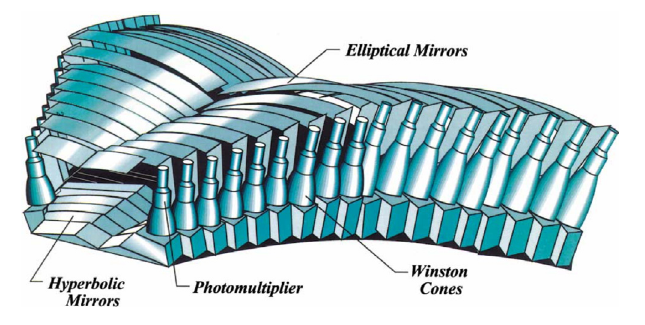
\includegraphics[width=\linewidth]{213ltcc.png}}
        \caption[LTCC Mirror System]
        {Layout and components of the optical mirror system within each LTCC box from the design model.}
        \floatfoot{Source: \href{https://jlab.org/physics/hall-b/clas12}{CLAS12 wiki}.}
        \label{fig::11.213::ltcc}
    \end{wrapfigure}

    The drift chambers are capable of detecting ionising particles with momenta above $200 ~\text{MeV}/\text{c}$, with a momentum resolution of $\Delta p/p$ less than $0.5\%$. This level of resolution corresponds to a track momentum resolution of $3\%$ to $5\%$.
    The high precision in momentum measurements allows for accurate reconstruction of particle trajectories and precise determination of their momenta, which is crucial for the physics analysis in the experiment \cite{mestayer2020}.

    % !TEX root = ../main.tex
\paragraph{Low Threshold Cherenkov Counter (LTCC)}
    The LTCC system is used for charged pion and kaon detection at momenta between $3.5$ and $9 ~\text{GeV}$.
    The LTCC system consists of boxes shaped like truncated pyramids.
    Four of the six sectors of CLAS12 are equipped with one LTCC box.
    Each LTCC box contains 108 lightweight mirrors with composite backing structures, 36 Winston light-collecting cones, 36 125-mm diameter PMTs, and 36 magnetic shields.
    The LTCC boxes are filled with heavy C4 F10 radiator gas.

    \begin{wrapfigure}{l}{0.50\textwidth}
        \centering\frame{
        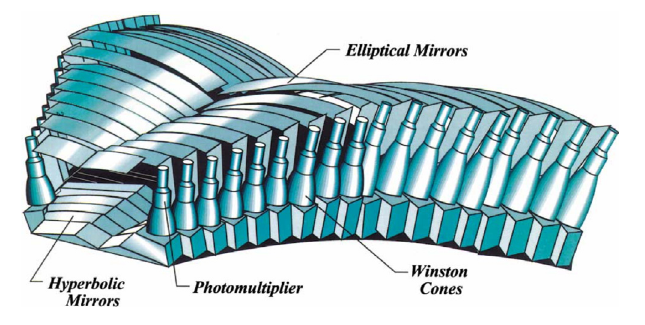
\includegraphics[width=\linewidth]{213ltcc.png}}
        \caption[LTCC Mirror System]{Layout and components of the optical mirror system within each LTCC box from the design model.}
        \label{fig::ltcc}
    \end{wrapfigure}

    The LTCC was a detector used in CLAS, which as part of the 12 GeV upgrade was refurbished to provide higher efficiency for charged pion and kaon detection.
    This was done by increasing the volume of the radiator gas, refurbishing the elliptical and hyperbolic mirrors with new coatings, and improving the sensitivity of the PMTs to Cherenkov light.
    The sensitivity improvement was achieved by coating their entrance windows with wavelength shifting material that absorbs ultraviolet (UV) light at wavelength below $300 ~\text{nm}$ and re-emits two back-to-back photons at larger wavelength \cite{ungaro2020}.
    A drawing from the design model of the LTCC can be seen in Figure \ref{fig::ltcc}.

    % !TEX root = ../main.tex
\paragraph{Forward Time-of-Flight (FTOF)}
    \begin{wrapfigure}{r}{0.50\textwidth}
        \centering\frame{
        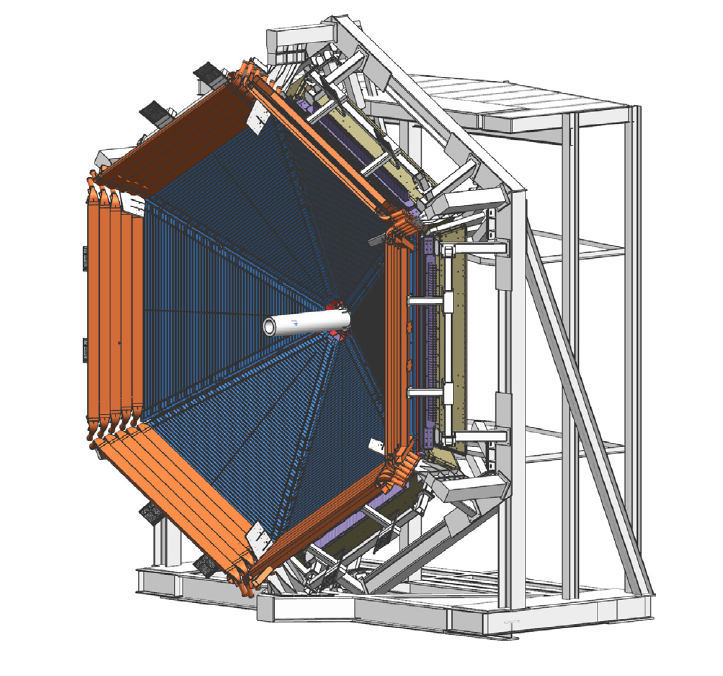
\includegraphics[width=\linewidth]{214ftof.png}}
        \caption[FTOF]{Render of the Forward Carriage with the FTOF system showing the panel-1b counters on the inside (dark blue), and the panel-2 counters on the outside (bronze).
        The panel-1a counters are located immediately downstream of the panel-1b counters and are not visible in the render.
        Part of the PCAL is visible downstream of the FTOF panels.
        Source: \hyperlink{jlab.org/physics/hall-b/clas12}{CLAS12 wiki}.}
        \label{fig::ftof}
    \end{wrapfigure}

    The FTOF system in CLAS12 is designed to measure the time-of-flight of charged particles emerging from the target during beam operation.
    It consists of six sectors of plastic scintillators with double-sided PMT readout.
    Each sector is divided into three arrays of counters separated into panels.
    Panel-1a has 23 counters, panel-1b has 62 counters, and panel-2 has 5 counters.
    The FTOF system is designed to provide excellent timing resolution for particle identification and good segmentation for flexible triggering options.
    The detectors cover a polar angle range from $5\degree$ to $45\degree$, spanning $50\%$ in azimuth at $5\degree$ and $90\%$ at $45\degree$.
    The lengths of the counters vary across the panels, ranging from $32.3 ~\text{cm}$ to $376.1 ~\text{cm}$ in panel-1a, from $17.3 ~\text{cm}$ to $407.9 ~\text{cm}$ in panel-1b, and from $371.3 ~\text{cm}$ to $426.2 ~\text{cm}$ in panel-2.

    The timing resolution achieved in the FTOF system is $125 ~\text{ps}$ in panel-1a, $85 ~\text{ps}$ in panel-1b, and $155 ~\text{ps}$ in panel-2.
    This timing resolution allows for precise measurements of the particle's time-of-flight, which is crucial for particle identification purposes \cite{carman2020ftof}.
    A render of the FTOF detector can be seen in Figure \ref{fig::ftof}.

    % !TEX root = ../main.tex
\paragraph{Ring Imaging Cherenkov Detector (RICH)}
    To improve particle identification in the momentum range of $3 - 8 ~\text{GeV}$, a RICH detector was incorporated into one of the CLAS12 sectors, replacing the corresponding LTCC sector.
    The RICH detector enhances CLAS12's capabilities in separating kaons from pions.

    The RICH detector consists of aerogel radiators, visible light photon detectors, and a focusing mirror system.
    The focusing mirror system is designed to reduce the instrumented detection area to $1 ~\text{m}^2$.
    Multi-anode PMTs are used as the photon detectors, providing the necessary spatial resolution and matching the aerogel Cherenkov light spectrum in the visible and near-UV region.

    For forward scattered particles with momenta between $3$ and $8 ~\text{GeV}$ and angles up to $13\degree$, a proximity imaging method is employed.
    This method utilises a thin ($2 ~\text{cm}$) aerogel radiator for direct Cherenkov light detection.

    For particles with larger incident angles between $13\degree$ and $25\degree$ and momenta ranging from $3$ to $6 ~\text{GeV}$, a different configuration is used.
    The Cherenkov light is produced by a thicker aerogel layer of $6 ~\text{cm}$ and focused by a spherical mirror.
    The light then undergoes two additional passes through thin radiator material and is reflected by planar mirrors before detection \cite{contalbrigo2020}.
    This setup enables efficient particle identification in this momentum and angular range.

    % !TEX root = ../main.tex
\paragraph{Electromagnetic Calorimeters (ECAL)}
\label{par::ecal}
    The CLAS12 detector package incorporates the existing electromagnetic calorimeter (EC) from the CLAS detector and adds a new pre-shower calorimeter (PCAL) upstream of the EC.
    Together, they form the ECAL, which is primarily used for the identification and kinematical reconstruction of electrons, photons, and neutrons.

    The ECAL consists of six modules, with the PCAL and EC divided into two parts each along the direction from the target.
    These parts are known as EC-inner (ECIN) and EC-outer (ECOU) and are read out separately.
    They provide longitudinal sampling of electromagnetic showers and also help improve particle identification through hadronic interactions.

    Each module has a triangular shape and is composed of 54 layers of scintillators.
    The scintillators are 1 cm thick and segmented into strips that are 4.5 cm wide for PCAL and 10 cm wide for EC, fitted between 2.2-mm-thick lead sheets.
    The total thickness of the calorimeters corresponds to approximately 20.5 radiation lengths.
    The scintillator layers are grouped into three readout views, with 5/5/8 layers per view for PCAL/ECIN/ECOU, respectively.
    This arrangement allows for spatial resolutions of less than 2 cm for energy clusters.

    To transmit the light signals from the scintillators, flexible optical fibers are used to route the light to the corresponding PMTs \cite{asryan2020}.

    % !TEX root = ../main.tex
\paragraph{Forward Tagger (FT)}
    The FT is an extension of the CLAS12 detector that allows for the detection of electrons and photons at very forward polar angles, specifically ranging from $2.5\degree$ to $4.5\degree$.
    By detecting forward-scattered electrons, the FT enables electroproduction experiments at low photon virtuality $Q^2$, providing a high-intensity, linearly polarized, quasi-real photon beam with energy tagging.
    This setup is particularly suitable for hadron spectroscopy studies.

    The FT consists of three main components: the FTCal (calorimeter), the FTTrk (micro-strip gas tracker), and the FTHodo (hodoscope).
    The FTCal utilises 332 lead-tungstate ($\text{PbWO}_4$) crystals to identify electrons, measure the energy of electromagnetic showers, and provide fast trigger signals.
    The FTTrk, located in front of the FTCal, is responsible for measuring the scattering angles of charged particles.
    The FTHodo, a scintillator detector, assists in the separation of electrons and high-energy photons.

        \begin{wrapfigure}{l}{0.50\textwidth}
            \centering\frame{
            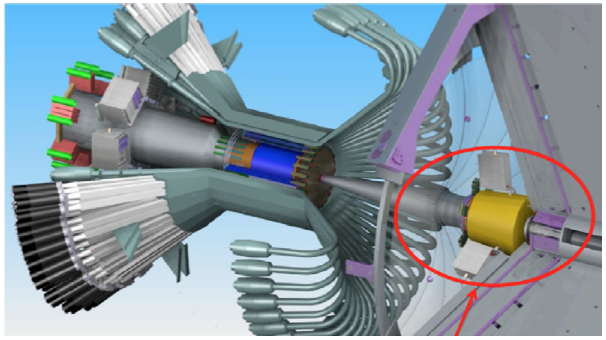
\includegraphics[width=\linewidth]{217ft.png}}
            \caption[FT]{The Forward Tagger system circled downstream of the CD in front of the torus magnet warm bore entrance.
            Source: \hyperlink{jlab.org/physics/hall-b/clas12}{CLAS12 wiki}.}
            \label{fig::11.217::ft}
        \end{wrapfigure}

    During beam operations, a conical tungsten shielding pipe is placed in front of the FT to absorb M\o ller electrons and low-energy photons generated by beam interactions with the target and downstream materials.
    This shielding not only protects the FT and Forward Detectors from electromagnetic background but also ensures compatibility with the FT acceptance.
    This configuration, referred to as ``FT-ON'', allows the FT to detect both electrons and photons, expanding the detection capabilities of CLAS12.

    Alternatively, when the FT is not required for the specific physics program, the FT detectors can be turned off, and additional shielding elements are installed in front of the FT, covering up to $4.5\degree$ of polar angle.
    This modified configuration, known as "FT-Off," reduces accidental background by one-third under the same beam conditions, enabling higher luminosity data acquisition with CLAS12 by mitigating background interference from the DC R1 chambers \cite{acker2020ft}.


    % !TEX root = ../main.tex
\subsubsection{Central Detector (CD)}
\label{11.220::central_detector}
    In the CD, particles scattered from the target within the polar angle range of $35\degree$ to $125\degree$ are detected.
    The CD consists of various detectors that provide particle identification and tracking capabilities.
    Charged particles are detected in the Central Vertex Tracker (CVT) and the Central Time-of-Flight (CTOF) detector.
    Neutron detection is provided by the Central Neutron Detector (CND), which is located radially outside of the CVT and the CTOF.
    All detectors have full coverage in the azimuthal angle.

    % !TEX root = ../main.tex
\paragraph{Central Vertex Tracker (CVT)}
    The CVT system is an integral part of the CD.
    It is primarily used for measuring the momentum and determining the vertex position of charged particles scattered from the target.

    The CVT system is located inside the solenoid magnet, as depicted in Figure \ref{fig::11.221::cvt}.
    It consists of two distinct detectors: the SVT and the Barrel Micromegas Tracker (BMT).

    The SVT system is composed of three regions, each equipped with double-sided modules of silicon sensors.
    The regions have different numbers of modules: 10, 14, and 18, respectively.
    These silicon sensors are instrumented with a digital Application-Specific Integrated Circuit (ASIC) readout.
    The readout pitch, which refers to the distance between adjacent readout channels, is approximately 156 micrometers.
    The SVT system comprises 21,504 channels \cite{antonioli2020}.

    \begin{wrapfigure}{r}{0.50\textwidth}
        \frame{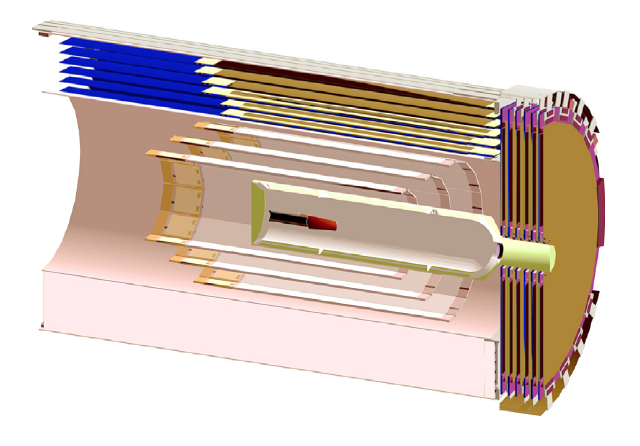
\includegraphics[width=\linewidth]{221cvt.png}}
        \caption[Central Vertex Tracker (CVT)]
        {Render of the Central Vertex Tracker (CVT).
        From the inside, the figure shows the target cell and vacuum chamber, the three double layers of the SVT, followed by the six layers of the BMT.
        The beam enters from the left.
        The six Forward Micromegas Tracker (FMT) layers are shown at the downstream end at the right.}
        \floatfoot{Source: \href{https://jlab.org/physics/hall-b/clas12}{CLAS12 wiki}.}
        \label{fig::11.221::cvt}
    \end{wrapfigure}

    The BMT is composed of three layers of strips aligned along the beamline and three layers of circular readout strips around the beamline, totalling 15,000 readout elements.
    It significantly enhances momentum resolution and tracking efficiency.
    Each layer is divided azimuthally into three segments, providing $120\degree$ azimuthal coverage for each segment.
    The system is designed to operate at the full luminosity of $10^{35} \text{cm}^{-2}\text{s}^{-1}$ \cite{acker2020mvt}.

    % !TEX root = ../main.tex
\paragraph{Central Time-of-Flight}
    The CTOF system is utilised for the purpose of charged particle identification by measuring their time-of-flight (TOF) in the momentum range of approximately $0.3$ to $1.25 ~\text{GeV}$.
    It consists of 48 plastic scintillators with double-sided photomultiplier tube (PMT) readout.
    The PMTs are connected to the scintillators via 1.0-meter-long upstream and 1.6-meter-long downstream focusing light guides.
    These counters are arranged in a hermetic barrel configuration surrounding the target and the CVT, and they are aligned with the beam axis inside the 5 T solenoid magnet.

    To ensure accurate measurements, the PMTs are positioned within a region of 0.1 T fringe field of the solenoid magnet and are enclosed within a triple-layer dynamic magnetic shield.
    This shield minimises the internal magnetic field near the PMT photocathode, achieving a field strength of less than 0.2 G.
    The CTOF system is designed to provide a time resolution of 80 ps, enabling precise charged particle identification in the CLAS12 CD \cite{carman2020ctof}.

    For a visual representation of the CTOF system, you can refer to figure \ref{fig::ctof}.

    % !TEX root = ../main.tex
\paragraph{Central Neutron Detector (CND)}
    The Central Neutron Detector (CND) is a component of the CLAS12 Central Detector (CD) positioned radially outward of the CTOF system.
    Its primary function is to detect neutrons in the momentum range of $0.2$ to $1.0 \text{GeV}$ by measuring their TOF from the target and the energy deposition in scintillator layers.

    The CND is composed of three layers of scintillator paddles, with each layer containing 48 paddles.
    The paddles are coupled in pairs at the downstream end using semi-circular light guides.
    The signal generated in the scintillator paddles is read out at the upstream end by PMTs that are positioned outside the high magnetic field region of the solenoid magnet.

    To transmit the scintillation light, the scintillators are connected to 1-meter-long bent light guides, which ensure efficient light propagation to the PMTs for signal detection and readout.

    The combination of TOF measurements and energy deposition in the scintillator layers enables the CND to identify and detect neutrons within the specified momentum range in the CLAS12 CD \cite{chatagnon2020}.

    % !TEX root = ../main.tex
\paragraph{Back Angle Neutron Detector (BAND)}
\label{par::band}
    \begin{wrapfigure}{r}{0.49\textwidth}
        \centering\frame{
        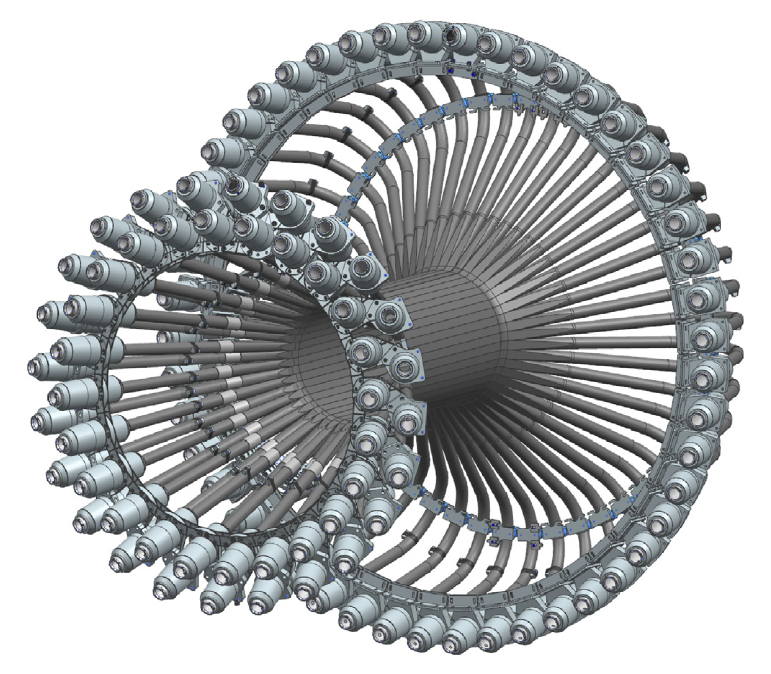
\includegraphics[width=\linewidth]{222ctof.png}}
        \caption[Central Time-of-Flight]{Render of the Central Time-of-Flight.
        The render shows CTOF's 48 scintillator bars outfitted with light guides, PMTs, and magnetic shields at both ends of each counter.
        Source: \hyperlink{https://www.jlab.org/physics/hall-b/clas12}{CLAS12 wiki}.}
        \label{fig::ctof}
    \end{wrapfigure}

    The CLAS12 spectrometer includes the BAND as a dedicated detector for neutron detection at backward angles.
    Positioned 3 metres upstream of the target, the BAND is designed to detect backward-scattered neutrons with momenta ranging from 0.25 to 0.7 GeV.

    The BAND detector consists of 18 horizontal rows and five layers of scintillator bars.
    Each scintillator bar is equipped with PMT readout on both ends to measure the TOF of neutrons originating from the target.
    Additionally, there is an extra 1 cm scintillation layer specifically designed to veto charged particles, ensuring that only neutrons are detected.

    Covering a polar angle range from $155\degree$ to $175\degree$, the BAND detector achieves a design neutron detection efficiency of $35\%$.
    It also provides a momentum resolution of approximately $1.5\%$, allowing for precise measurements of the momentum of the detected neutrons \cite{segarra2020}.

    By utilising the BAND detector, the CLAS12 spectrometer is capable of detecting and characterising backward-scattered neutrons, providing valuable information for various physics studies and experiments conducted at CLAS12.


    % % !TEX root = ../main.tex
\subsubsection{Offline Reconstruction}
\label{11.230::offline_reconstruction}
% --+ CLARA +-------------------------------------------------------------------
    The CLAS12 reconstruction and analysis process is facilitated by a data-stream processing framework called CLARA.
    CLARA adopts a service-oriented architecture, allowing the construction of software applications using micro-services that are connected via data-stream pipes \cite{gyurgyan2016}.

    In this framework, each service plays a specific role.
    It receives input data, processes it according to its functionality, and produces output data.
    The input and output data are organised in tabular structures known as ``banks'', which are configured by the service developer to match the specific requirements of the service.

    The services within CLARA form a data-flow path, where the output of one service becomes the input for the next service in the sequence.
    This design enables a flexible and versatile data processing application, as each service can be individually improved or replaced without necessitating structural changes to the framework.

    To ensure consistency and modularity, the CLAS12 services are extensions of an abstract reconstruction engine.
    This engine provides common components such as initialisation and event processing methods, reducing the development complexity of individual micro-services and enforcing a uniform structure throughout the framework.

    By leveraging the CLARA framework, the CLAS12 experiment benefits from a modular and adaptable data processing pipeline, allowing for efficient reconstruction and analysis of the collected data.
    The service-oriented architecture and data-stream processing approach contribute to the flexibility, scalability, and maintainability of the CLAS12 software framework.

    \begin{figure}[b!]
        \centering\frame{
        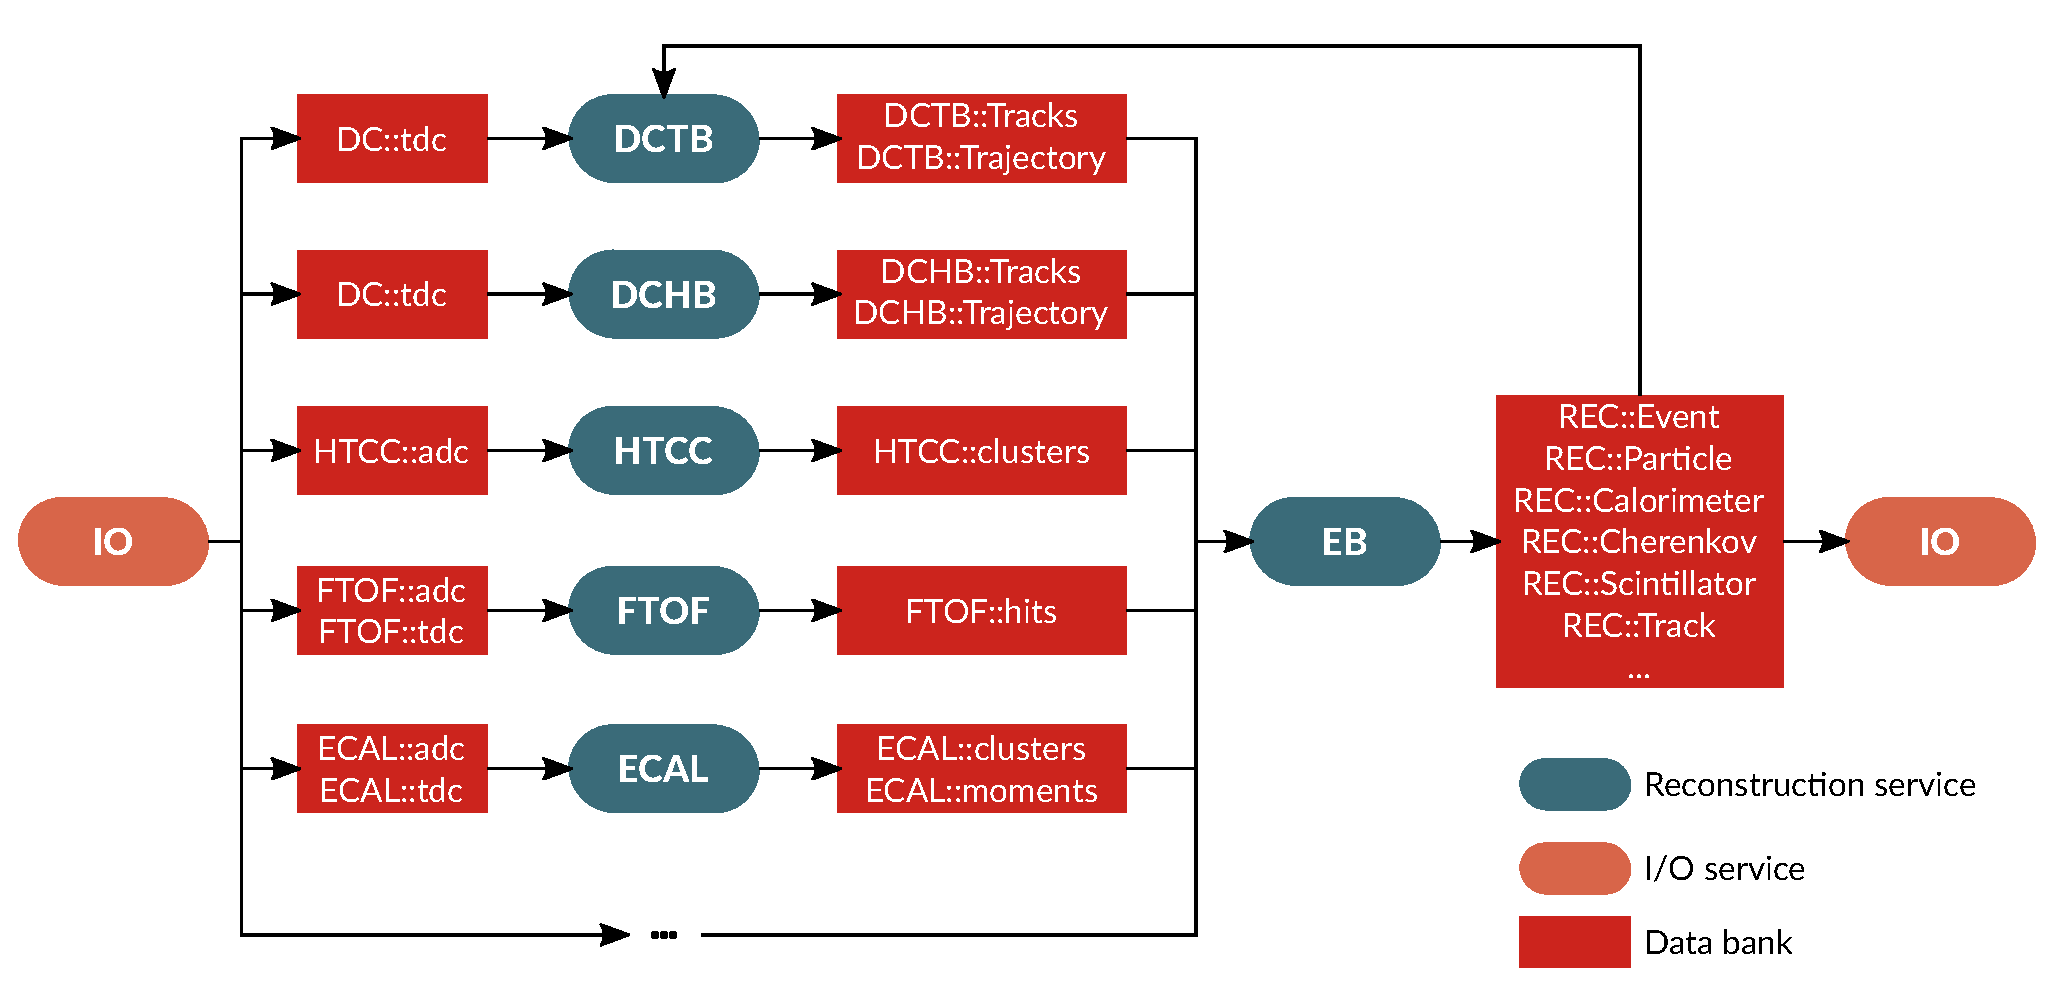
\includegraphics[width=\textwidth]{230recon_chain.pdf}}
        \caption[CLAS12 Reconstruction Chain.]{Graphical representation of the CLAS12 interdependencies between services and banks.
        The I/O service reads events from the input file and distributes them to the reconstruction services chain for processing.
        Each service reads the relevant banks, applies the reconstruction algorithm, and provides output banks that are passed to the next service in the chain.
        The Event Builder (EB) service is executed as last in the chain; it collects the relevant banks from all CLAS12 subsystems services and produces event, particle, and detector response banks that are written to the output file.
        Source: Own elaboration, using \href{https://inkscape.org/}{Inkscape}.}
        \label{fig::11.230::recon_chain}
    \end{figure}

% --+ CLAS12 reconstruction +---------------------------------------------------
    The CLAS12 data reconstruction process involves data reader services that access decoded detector data stored in banks.
    Each entry in the bank represents a decoded detector hit and contains information such as sector, layer, component, order, and digitised data like signal charge, amplitude, time, or pedestal.

    During the decoding stage, similar bank structures are created for various quantities required for event reconstruction, including hits, clusters, and tracks.
    Reconstruction algorithms specific to each CLAS12 subsystem fill these banks.
    The data persistence service appends and writes these banks to a file for later analysis.

    The reconstruction algorithms are implemented as services that operate on input banks and produce output banks, which are then passed to subsequent algorithms in the reconstruction chain.
    The order in which the services are chained reflects the overall sequence of CLAS12 event reconstruction and the dependencies between subsystems.

    The first step is the reconstruction of charged particle tracks in the Central and Forward Detector tracking systems, based on the recorded hit positions in the respective detectors.
    This process is known as ``hit-based'' tracking.

    Simultaneously, hits recorded in other detectors are processed to reconstruct the energy and time of the associated particle interactions.
    The Event Builder (EB) service matches these reconstructed quantities with the tracks based on position and time information.
    Hits that are not matched to any track are retained as neutral particle candidates.
    The EB also determines the event ``start time'' and identifies the reconstructed particles.

    Once the event start time is determined, a second iteration of forward tracking, known as ``time-based'' tracking, can be performed.
    This iteration incorporates the drift times in the Drift Chambers, providing improved tracking precision \cite{ziegler2020}.

    An overview of the composition of reconstruction application services, depicting the dependencies between the services, can be found in Figure \ref{fig::11.230::recon_chain}.

    % !TEX root = ../main.tex
\paragraph{Tracking}
% --+ Introduction +------------------------------------------------------------
    \begin{wrapfigure}{r}{0.50\textwidth}
        \centering\frame{
        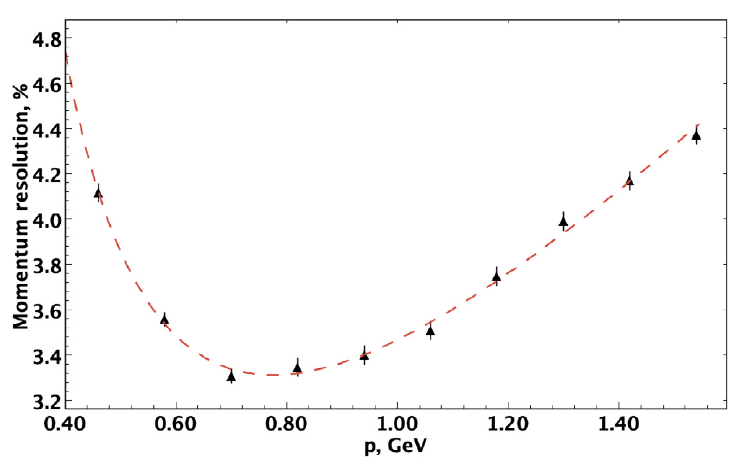
\includegraphics[width=\linewidth]{231cvt_pres.png}}
        \caption[CVT momentum resolution vs. momentum.]{Momentum resolution vs. momentum of simulated protons in the CVT without background.
        Source: \cite{ziegler2020}.}
        \label{fig::11.231::cvt_p_resolution}
    \end{wrapfigure}

    In the CLAS12 event reconstruction, charged particle tracking plays a crucial role and is divided into two main regions: the forward region and the central region.

    In the forward region, charged particles are bent either inward or outward from the beamline by the torus magnet, depending on their charge.
    The magnetic field strength varies along the bending path, with an integral magnetic field ($\int Bdl$) ranging from $2 \text{Tm}$ at $5\degree$ to $0.5 \text{Tm}$ at $40\degree$.
    The forward tracking system responsible for tracking in this region consists of two components: the Forward MicroMegas Tracker (FMT) and the Drift Chambers (DC).

    In the central region, charged tracks are curved into helices by the strong $5 \text{T}$ solenoidal magnetic field.
    The central tracking system comprises the Silicon Vertex Tracker (SVT) and the Barrel MicroMegas Tracker (BMT), which together form the Central Vertex Tracker (CVT).

    These tracking systems in both the forward and central regions use sophisticated detectors to measure the position of charged particle hits, allowing for the reconstruction of particle trajectories.
    By combining information from these detectors and utilising the magnetic field information, the tracking algorithms reconstruct the paths of charged particles, enabling precise determination of their momenta and vertices.

% --+ Reconstruction +----------------------------------------------------------
    In both the forward and central tracking systems, track reconstruction involves two main steps: pattern recognition and track fitting.
    The first step is to identify hits, which are the recorded signals corresponding to a particle passing through a specific detector component.
    These hits are transformed from electronic signals into the position of the track within the geometry of the detector subsystem.

    \begin{wrapfigure}{r}{0.50\textwidth}
        \centering\frame{
        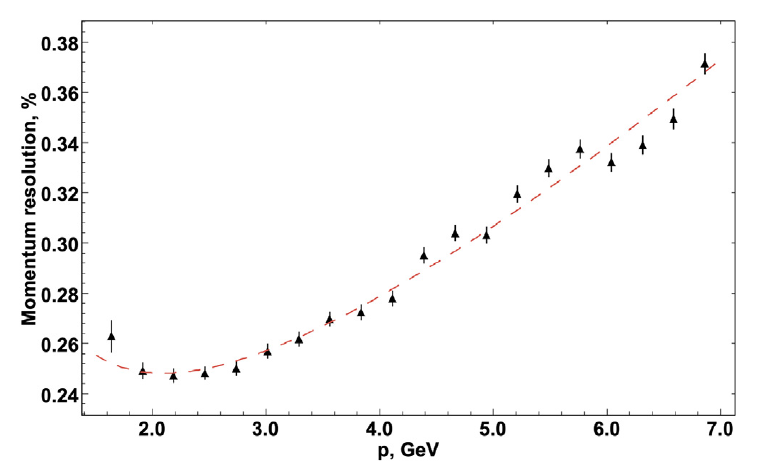
\includegraphics[width=\linewidth]{231dc_pres.png}}
        \caption[DC momentum resolution vs momentum.]{Momentum resolution vs. momentum in the DC evaluated using pions simulated at $\theta = 15\degree \pm 5\degree$ and at $\phi = 0 \pm 5\degree$ without background.
        Source: \cite{ziegler2020}.}
        \label{fig::11.231::dc_p_resolution}
    \end{wrapfigure}

    A hit is defined as a geometric object that represents a detector element.
    For example, in the central tracker, a hit can be represented by a line corresponding to a strip in the detector.
    These hit objects serve as the input for the pattern recognition algorithms.

    \begin{figure}[t]
        \centering\frame{
        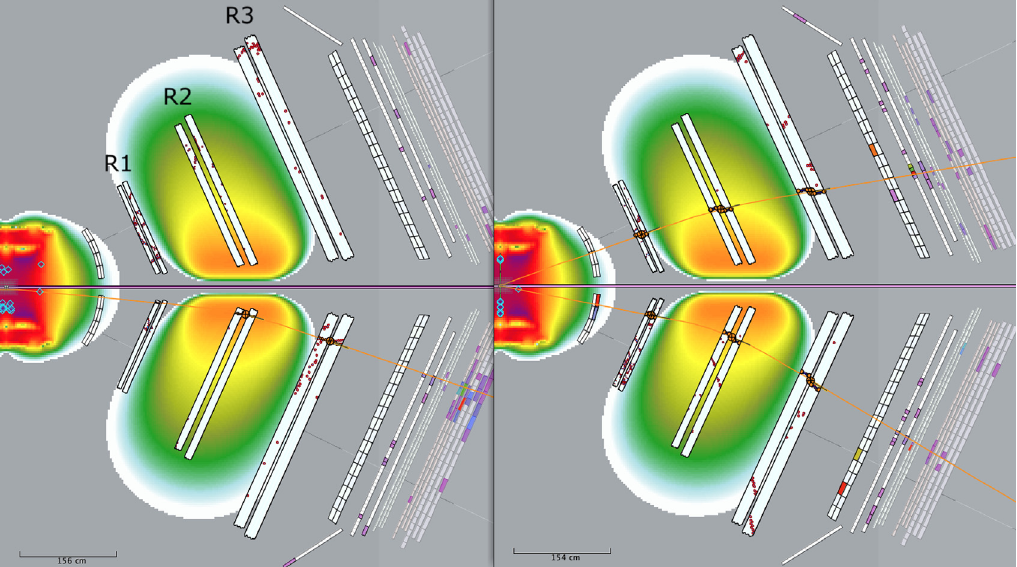
\includegraphics[width=\textwidth]{231ced_event.png}}
        \caption[Particle going through DC.]{Views from CLAS12 Event Display (ced) of charged particle tracks in the DC showing cut-views to highlight different pairs of sectors of the CLAS12 Forward Detector.
        The coloured detector elements are the registered hits and the orange lines are the result of track reconstruction using the hits in the DC.
        The coloured areas about the detectors represent the regions of magnetic field from the torus and the solenoid.
        In these views the beam is incident from the left and the target is located in the middle of the solenoid (at the left edge of the image).
        Source: CED render.}
        \label{fig::ced_event}
    \end{figure}
    Pattern recognition involves identifying clusters of hits and determining the spatial coordinates and corresponding uncertainties for the hits and clusters.
    During the pattern recognition stage, hits that are consistent with belonging to a trajectory, such as a particle track, are identified.
    This set of hits is then fitted to the expected trajectory, considering their uncertainties and incorporating knowledge of the detector material and the detailed magnetic field map.
    Figure \ref{fig::ced_event} illustrates a particle passing through the DC.

% --+ Performance +-------------------------------------------------------------
    The momentum resolutions in the central and forward trackers, as a function of momentum, are shown in Figures \ref{fig::11.231::cvt_p_resolution} and \ref{fig::11.231::dc_p_resolution}, respectively.
    The distributions are fitted with a function of the form $\sqrt{a + bx^2 + c/(1 + d/x^2)}$.
    In both distributions, the degradation of resolution at low momentum is attributed to multiple scattering effects.
    Furthermore, the resolution deteriorates as momentum increases beyond a minimum, primarily because of poorer track curvature resolution.

    For central tracking, a simulated proton sample with momenta ranging from $0.5$ to $2.5 \text{ GeV}$ yields an average CVT reconstruction efficiency of $87.3\%$.
    A slight decrease in efficiency is observed for tracks with momenta below $600 \text{ MeV}$.
    The increased curvature of low transverse momentum ($\text{p}_\perp$) tracks leads to a rise in inefficiency due to acceptance effects.
    The primary source of inefficiency stems from the gaps between the sensitive volumes of the BMT and SVT detectors.

    Regarding forward tracking, the momentum resolution in the DC is evaluated using tracks simulated at $\theta = 15\degree \pm 5\degree$ and $\phi = 0 \pm 5\degree$.
    This range ensures that the majority of tracks fall within the sensitive volume.
    Moreover, the DC momentum resolution exhibits correlation with the polar angle since track curvature is determined by the magnetic field intensity, which is higher at lower angles in the torus field.
    These resolutions are obtained from a Monte Carlo sample that excludes out-of-time backgrounds or misalignments of the tracking volumes \cite{ziegler2020}.

    % !TEX root = ../main.tex
\paragraph{Particle Identification}
% --+ PDG PID +-----------------------------------------------------------------
    The Particle Identification (PID) numbering scheme described here was initially introduced by the Particle Data Group (PDG) in 1988 \cite{yost1988}.
    Its purpose is to facilitate communication and data exchange between different generators, simulators, and analysis packages employed in particle physics.
    The system underwent subsequent revisions and adaptations in 1998 to allow for the systematic inclusion of undiscovered and hypothetical particles \cite{particle1998}.
    The PID convention utilised in this thesis is based on the most up-to-date version available at the time of writing, as referenced from the 2020 Review of Particle Physics by the PDG \cite{particle2020}.

% --+ The Event Builder +-------------------------------------------------------
    The EB is a crucial component within the reconstruction chain, serving multiple functions:
    \begin{itemize}
        \item
            It gathers information from upstream services.
        \item
            It correlates information from sub-detectors to form particles.
        \item
            It implements a general particle identification scheme.
        \item
            It organises the resulting information into a standardised and persistent data bank structure.
    \end{itemize}

    The EB service is executed twice using identical algorithms, first employing hit-based tracks and subsequently using time-based tracks.
    As mentioned previously, the results obtained from the hit-based EB are utilised to initialise time-based tracking.

% --+ Forming particles +-------------------------------------------------------
    In the definition of a reconstructed charged particle within CLAS12, the EB assumes that each reconstructed track in both the FD and the CD will be assigned an identification.
    The corresponding responses from the calorimeter, scintillator, and Cherenkov detectors are then associated with that particle based on geometric coincidences between the detector responses and the track.
    Matching criteria are established, which correspond to the resolution of each specific detector.
    The geometric matching process relies on the Distance of Closest Approach (DOCA) between the track and the detector response.

    A similar procedure is employed for the creation of neutral particles, with the distinction that the seeding is presently performed using unassociated responses from the ECAL for the FD and the CND (or the BAND) for the CD, instead of using tracks.

% --+ Event start time +--------------------------------------------------------
    A start time is assigned to the entire event and serves as the precise reference time for all time-based particle identification procedures.
    The determination of the start time relies on the optimal charged particle candidate in the FD with an associated timing response from the FTOF detector.

    The EB assigns the start time based on the highest energy electron detected in the ECAL.
    If no electron is found in the ECAL, the EB then searches for a positron in the ECAL.
    In the absence of any lepton candidates, the next track in the priority list is a forward-going positive track, which is assumed to be a positive pion ($\pi^+$).
    Finally, if no forward-going positive track is identified, the EB searches for a forward-going negative track, assumed to be a negative pion ($\pi^-$).
    When searching for $\pi^+$ or $\pi^-$ tracks, only the candidate with the highest momentum within each group is considered.

    A parallel event start time is determined from the FT system to facilitate physics analyses and triggers specifically for events where the primary scattered electron is at very forward angles within the FT.

    In such cases, all combinations of charged particles in both the FT and the FD are taken into account.
    The particle in the FT is assumed to be an electron, while all possible hadron mass hypotheses are considered for the FD tracks.
    The combination that exhibits the best time coincidence is selected, and the timing of the resulting FT electron is used to assign the start time.

    A correction to the start time is subsequently applied using the RF signal from the accelerator, in conjunction with the reconstructed event vertex position.
    This correction effectively aligns the event start time with the most accurate measurement of the beam-bunch arrival time at the target.

    The uncorrected measured vertex time of a particle, denoted as $t_v$, can be expressed as follows
    \begin{equation*}
        t_v = t - \frac{P_L}{\beta c},
    \end{equation*}

    Here, $t$ represents the measured time response (e.g., in a scintillator), $P_L$ is the path length between the primary interaction vertex and the corresponding response, and $\beta c$ denotes the speed of the particle.

    Next, we calculate the time difference $\Delta t_{RF}$ between $t_v$ and the nearest beam bunch using the following formula
    \begin{equation*}
        \Delta t_{RF} = t_v + \frac{z_0 - z_v}{c} - t_{RF} - \frac{N}{2f_{RF}},
    \end{equation*}

    In this equation, $z_v$ represents the $z$-coordinate of the event vertex position, $z_0$ is the reference position calibration at the center of the target, and $c$ denotes the speed of light in vacuum.
    $t_{RF}$ and $f_{RF}$ correspond to the measured and calibrated RF time and frequency of the accelerator.
    These values can either be $2.004 \text{ ns}$ and $249.5 \text{ MHz}$, or $4.008 \text{ ns}$ and $499 \text{ MHz}$, respectively.
    During the reconstruction process, these values are obtained from the Run Conditions Database.

    \begin{wrapfigure}{r}{0.49\textwidth}
        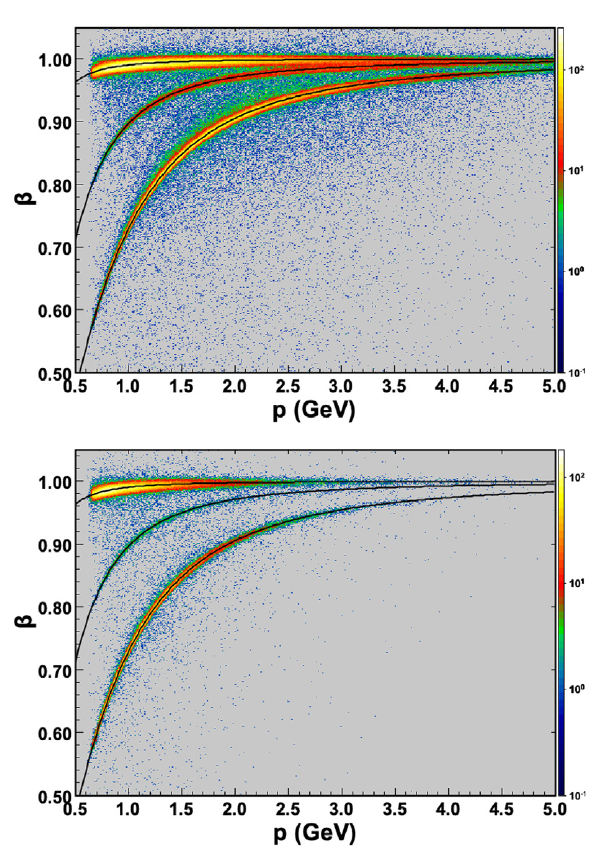
\includegraphics[width=\linewidth]{232pos_pid.png}
        \caption[Particle $\beta$ vs. momentum for positively charged tracks]
        {Particle $\beta$ vs. momentum from simulation data for positively charged tracks with their start time from an electron in the FD (top plot) or in the FT (bottom plot).}
        \floatfoot{Source: \cite{ziegler2020}.}
        \label{fig::11.232::positive_pid}
    \end{wrapfigure}

    Subsequently, the time can be further corrected to the nearest beam bunch using the equation
    \begin{equation*}
        \Delta t^\prime_{RF} = \text{mod}\left(\Delta t_{RF}, \frac{1}{f_{RF}}\right) - \frac{1}{2f_{RF}},
    \end{equation*}

    This correction allows for RF-correction to $t_v$. Thus, we obtain a final RF- and vertex-corrected start time for the event, defined as
    \begin{equation*}
        t' = t_v - \Delta t^\prime_{RF}.
    \end{equation*}

% --+ Charged particle identification +-----------------------------------------
    The subsequent step involves a basic particle identification scheme designed to be flexible enough to accommodate various physics analyses while retaining essential information for future refinement of the criteria.

    For charged particles, the identification process begins by utilising calorimetry and Cherenkov information to positively identify $e^-/e^+$ candidates in the FD.
    If the measured energy deposition aligns with the expected sampling fraction of the ECAL and the photoelectron response from the HTCC aligns with $\beta \sim 1$, the particle is assigned as an $e^-$ or $e^+$ based on the sign of curvature determined from forward tracking with the DC in the presence of the torus magnetic field.

    The remaining charged particles are then assumed to be hadrons and are assigned an identity solely based on timing information.
    The $p, K, \pi$ candidate with the smallest time residual is selected.
    This time residual is calculated as the difference between the measured flight time of the particle and the flight time computed for a specific mass hypothesis.

    Figure \ref{fig::11.232::positive_pid} presents the $\beta$ vs. momentum distributions for forward-going positively charged hadrons reconstructed using data from the FTOF and DC subsystems.
    The electron is reconstructed either in the FD (top) or in the FT (bottom).
    The computed curves for different mass hypotheses are superimposed on the distributions.

    \begin{wrapfigure}{r}{0.50\textwidth}
        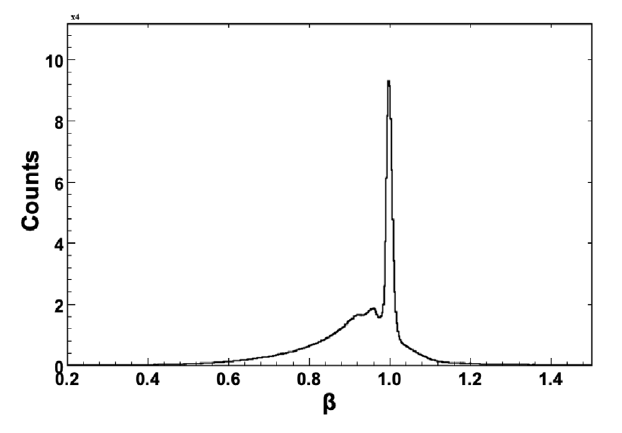
\includegraphics[width=\linewidth]{232n_gamma.png}
        \caption[$\beta$ distribution of neutrals]
        {$\beta$ distribution for neutral particles as measured by the ECAL from simulation data, showing a sharp peak at $\beta = 1$ from photons and a broader, slower distribution from neutrons.}
        \floatfoot{Source: \cite{ziegler2020}.}
        \label{fig::11.232::neutrons_and_gamma}
    \end{wrapfigure}

% --+ Neutral particle identification +-----------------------------------------
    To identify neutral particles, the analysis assumes the presence of only neutrons and photons, distinguished solely by timing and topological information.
    In the FD, the identification is based on the ECAL, while in the CD, it relies on the CND.
    The reconstructed cluster positions of these detectors are used to calculate the particle's travel path from the event vertex, assuming a straight-line trajectory.

    If the measured $\beta$ value is close to $1$, the particle is identified as a photon; otherwise, it is identified as a neutron.
    For photons in the FD, the momentum is determined from the deposited energy and the ECAL sampling fraction \cite{asryan2020}.
    For neutrons, the momentum is assigned based on the measured $\beta$, assuming the mass of a neutron.

    Figure \ref{fig::11.232::neutrons_and_gamma} illustrates an example of the reconstructed $\beta$ values for neutral particles in the FD, demonstrating the separation between photons and neutrons.

% --+ Particle identification performance +-------------------------------------
    A particle identification quality factor, represented as a signed-$\chi^2$ or pull, is assigned based on the contributions from individual detector subsystem responses and their resolutions.
    For $e^-/e^+$ identification, the resolution-normalised distance from the expected ECAL sampling fraction is utilised, while for charged hadrons, the resolution-normalised time difference is employed.
    The resulting information is organised into standardised output bank structures for physics analysis.
    This includes the particle four-vectors, associated detector responses, and global event information such as beam RF and helicity details.

    The accuracy of the currently implemented particle identification algorithm can be estimated by comparing the assigned particle identification with the true identification in Monte Carlo simulations.
    Table \ref{tab::11.232::reconstruction_pid} presents the particle identification matrix for the FD (left) and CD (right).
    The values are derived from simulations involving electron-hadron or electron-photon pairs with hadron and photon momenta ranging from $1$ to $2.5 \text{ GeV}$ and electron momenta ranging from $1$ to $9 \text{ GeV}$.
    The diagonal elements represent cases where the particle is correctly identified, while the off-diagonal elements represent cases of misidentification \cite{ziegler2020}.

    \begin{table}
        \begin{tabularx}{\textwidth}{XXXXXXXXXXXXX}
            \multicolumn{7}{c}{\textit{Forward Detector Truth}} & & \multicolumn{5}{c}{\textit{Central Detector Truth}}  \\
            \cmidrule{1-7} \cmidrule{9-13}
                     & $e$      & $\pi$ & $K$  & $p$  & $n$  & $\gamma$ & &       & $\pi$    & $K$  & $p$  & $n$  \\
            \cmidrule{1-7} \cmidrule{9-13}
            $e$      & 0.98     &       &      &      &      &          & & $\pi$ & 0.84     & 0.14 & 0.00 &      \\
            $\pi$    &          & 0.93  & 0.10 & 0.00 &      &          & & $K$   & 0.11     & 0.80 & 0.01 &      \\
            $K$      &          & 0.03  & 0.80 & 0.00 &      &          & & $p$   & 0.03     & 0.04 & 0.95 &      \\
            $p$      &          & 0.03  & 0.02 & 0.98 &      &          & & $n$   &          &      &      & 0.11 \\
            \cmidrule{9-13}
            $n$      &          &       &      &      & 0.66 & 0.01     & &       &          &      &      &      \\
            $\gamma$ &          &       &      &      & 0.14 & 0.95     & &       &          &      &      &      \\
            \cmidrule{1-7}
        \end{tabularx}

        \caption[Particle identification matrix]
        {Particle identification matrix for the FD (left matrix) and CD (right matrix).
        The FD matrix is based on simulated hadrons and photons with momentum between $1$ and $2.5 \text{ GeV}$, and electrons up to $9 \text{ GeV}$.
        The CD matrix is based on simulated hadrons with momentum between $0.3$ and $1.1 \text{ GeV}$.
        The diagonal elements are correctly identified, while the off-diagonal elements are misidentified.
        Detector inefficiencies are included.}
        \label{tab::11.232::reconstruction_pid}
    \end{table}



    % !TEX root = ../main.tex
\subsection{RG-E Experiment} \label{ssec::rgeexperiment}
    The Run Group E (RG-E) experiment aims to measure the hadronic multiplicity ratio between different nuclei and deuterium.
    To do this, a double-target system is being built to be used in Hall B.
    The system will allow a precise comparison of a deuterium target and heavy solid targets, like carbon, aluminium, copper, tin, lead, etc.
    The experiment aims to further the understanding of hadronisation in the nuclear medium, colour transparency, and nuclear short-range correlations.

    During data acquisition, the cryo-target (deuterium) and a solid target will be exposed to the electron beam simultaneously.
    To minimise acceptance correction difference between targets, we aim to keep the distance between them as low as possible -- as long as we can differentiate between the targets in reconstruction.
    Part of this thesis' work involves improving offline reconstruction before the experiment to reduce this distance, which can be read in chapter \ref{sec::fmtalignmentandreconstruction}.

    Positioning both targets in the beam simultaneously allows us to cancel time-dependent systematic effects o increase the precision of final results.
    These include effects such as drifting gains and inefficient detector channels in the measurement of ratio-like observables.
    Then, since the target system will be in a vacuum, the switching between solid targets will need to be performed remotely.
    Additionally, it needs to be done as quickly as possible, to maximise the beam time of the experiment.

    The double target system will be able to switch between up to five different solid targets.
    The previous EG2 experiment performed on the former CLAS showed that the design of the double target system has significant advantages to reduce the systematic uncertainties \cite{hakobyan2008}.
    The principle of the target system is to have the solid targets installed on a carbon fibre band which slides on torlon rails.
    The band is moved by a piezo-motor, which -- like all other chosen materials -- is insensitive to magnetic fields.
    The design proposed can be seen in figure \ref{fig::double_target}.

    \begin{figure}[b!]
        \centering\frame{
        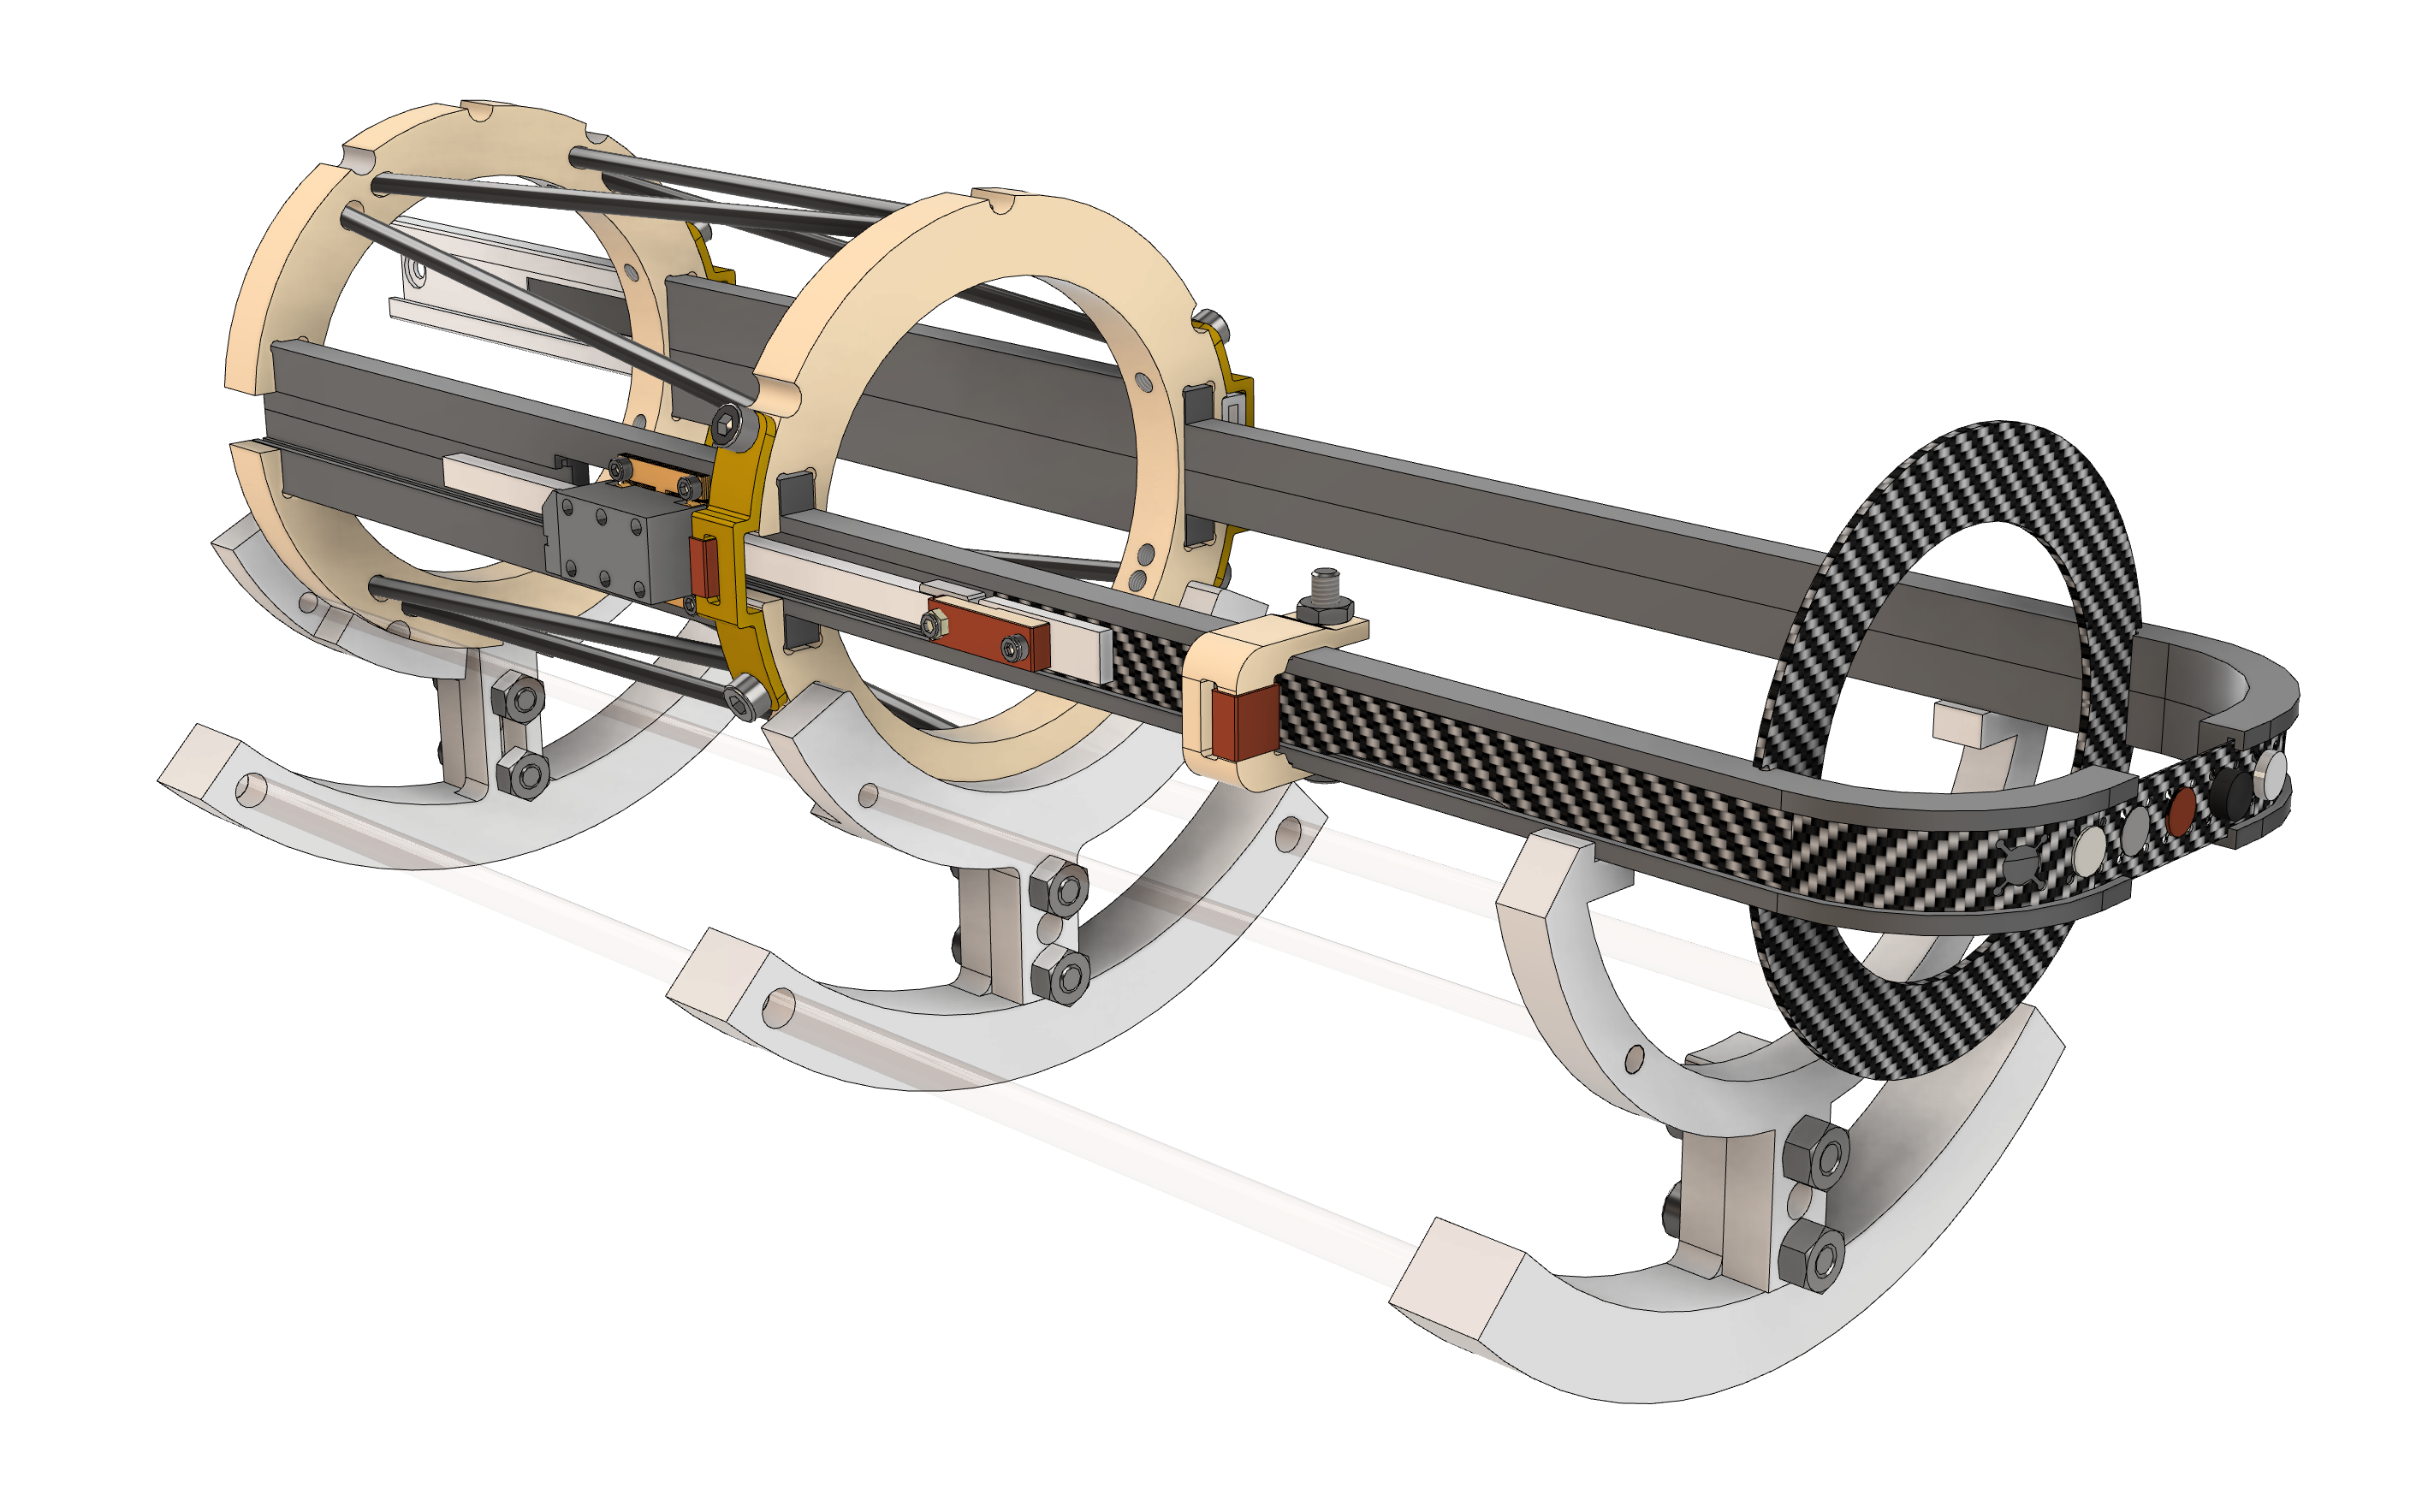
\includegraphics[width=\textwidth]{11experiment/img/30double_target.png}}
        \caption[Double-target system.]{Double-target system CAD render.}
        \label{fig::double_target}
    \end{figure}

    To ensure the adequate operation of the target, several tests were performed.
    These include movement under vacuum and high magnetic field, radiation hardness of the selected materials, and heat removal tests which secure that target remain far below melting point.

    % !TEX root = ../main.tex
\subsubsection{Slow Control System} \label{sssec::slowcontrolsystem}
% --+ What is slow control +----------------------------------------------------
    A modern experimental physics experiment usually involves many of moving parts and complex components that need constant monitoring and calibration.
    This is in addition to the constant data taking necessary.
    The process of automating this task is made via slow controls systems.
    These systems usually integrate a whole detector and experiment into one complex interface, allowing for easy access and maintenance.

% --+ What is EPICS +-----------------------------------------------------------
    The standard framework to do this in the context of HEP is the Experimental Physics and Industrial Control System (EPICS).
    EPICS was developed in the Los Alamos National laboratory (ANL) to provide data acquisition and control to this type of experiments.
    The framework provides a distributed process control that includes software communication, functional subsystems for data acquisition, supervisory control, closed loop control, channel archiving, and alarm management \cite{dalesio1991}.
    Like many HEP experiments, CLAS12's slow control system is based on EPICS \cite{boyarinov2020}.

% --+ EPICS installation on raspi +---------------------------------------------
    To allow the integration of the RG-E target on the CLAS12 slow controls system, an EPICS support module and Input / Output Controller (IOC) was developed by the author.
    This module wasn't made from scratch, as the motor developers made a generic support module for Galil motors \cite{farnswort2009}.
    This system proved to support all that was necessary for the movement of the RG-E target system, only requiring the removal of unnecessary features and the addition of database variables relevant to the experiment.
    % NOTE. This chapter doesn't involve the integration of thermocouples, as that is left as future work.

    The Process Variables (PVs) added to the EPICS module are listed, along with a short description of each.
    Each of these can be viewed and edited at the user-defined records database, which is at

    \begin{center}
        \texttt{\$EPICS\_BASE/support/galil/3-6/db/galil\_userdef\_records.template}.
    \end{center}

    \paragraph{Analog Input (\texttt{ai})}
        The normal use for this record type is to obtain an analog value from hardware and then convert it to engineering units \cite{stanley1998}.
        The record can also be used to write constants to be read from the database, such that they can be changed in runtime.

        \subparagraph{\texttt{DMC01:A\_curr\_pos}.}
            Current position of the band.
            Displayed at the GUI and used for internal calculations.

        \subparagraph{\texttt{DMC01:A\_home}.}
            Position of the home.
            Displayed at the GUI and used for calculations.

        \subparagraph{\texttt{DMC01:A\_pos\#}.}
            \# is a number from 1 to 7.
            Positions of each of the seven targets.
            Displayed at the GUI and used for calculations.

        \subparagraph{\texttt{DMC01:A\_lowlimit}.}
            Position of the low limit.
            If \texttt{DMC01:A\_curr\_pos} is lesser than this value, a major alarm is fired.

        \subparagraph{\texttt{DMC01:A\_highlimit}.}
            Position of the high limit.
            If \texttt{DMC01:A\_curr\_pos} is greater than this value, a major alarm is fired.

        \subparagraph{\texttt{DMC01:A\_tolerance}.}
            Equivalence tolerance for the position of each target and the position of the band.
            It defines a valid range around the target position.

        \subparagraph{\texttt{DMC01:COMMERR\_STATUS}.}
            Variable that is true when there's a communication error with the controller and false otherwise.
            Used for triggering a communication alarm.

        \subparagraph{\texttt{IOC01:SR\_i\_am\_alive}.}
            Variable that is true when the IOC is up and running, false otherwise.
            Used for triggering a communication alarm.

    \paragraph{Analog Output (\texttt{ao})}
        The normal use for this record type is to output values to digital-analog converters.
        The desired output can be controlled by either an operator or a state program, or it can be fetched from another record \cite{stanley1998}.

        \subparagraph{\texttt{DMC01:A\_go\_home}.}
            Command to move the band to the home position, as defined in \texttt{DMC01:A\_home}.

        \subparagraph{\texttt{DMC01:A\_go\_pos\#}.}
            Command to move the band to the position of target \#, as defined in \texttt{DMC01:A\_pos\#}.

    \paragraph{Calculation (\texttt{calc})}
        The calculation or ``Calc'' record is used to perform algebraic, relational, and logical operations on values retrieved from other records.
        The result of its operations can then be accessed by another record so that it can be used \cite{stanley1998}.
        In the context of the RG-E target, each calculation returns a number from 0 to 11.
        This number represent the state the target is in, and is later used by a Select PV.

        \subparagraph{\texttt{DMC01:A\_at\_pos\#}.}
            Calculation that checks if the band position is equal to that of target \# in \texttt{DMC01:A\_pos\#}, within the tolerance margin \texttt{DMC01:A\_tolerance}.
            If it is, it returns \#.
            Otherwise, it returns 0.

        \subparagraph{\texttt{DMC01:A\_at\_home}.}
            Calculation that checks if the band position is equal to the home position in \texttt{DMC01:A\_home}, within the tolerance margin defined by the tolerance.
            If it is, it returns 8.
            Otherwise, it returns 0.

        \subparagraph{\texttt{DMC01:A\_moving}.}
            Calculation that checks if the target is moving by checking the motor PV \texttt{DMC01:A.MOVN}.
            If it is, it returns 9.
            Otherwise, it returns 0.

        \subparagraph{\texttt{DMC01:A\_at\_lowlimit}.}
            Calculation that checks if the band position is lesser than the low limit \texttt{DMC01:A\_lowlimit}.
            If it is, it returns 10.
            Otherwise, it returns 0.

        \subparagraph{\texttt{DMC01:A\_at\_highlimit}.}
            Calculation that checks if the band position is greater than the high limit \texttt{DMC01:A\_highlimit}.
            If it is, it returns 11.
            Otherwise, it returns 0.

    \paragraph{Select (\texttt{sel})}
        The select record computes a value based on input obtained from up to 12 locations.
        By default, it is equal to the highest value among its input PVs \cite{stanley1998}.

        \subparagraph{\texttt{DMC01:A\_sel\_tgttype}.}
            This record returns the highest value between the previously defined calculations.
            Thus, it associates the values returned to a state of the target.
            By convention, this PV assumes that \emph{no more than one \texttt{calc} is greater than 0}.
            This assumptions holds as long as \texttt{DMC01:A\_tolerance} is not set higher than half the distance between targets and between the targets and the lower and higher limits.

    \paragraph{Multi-Bit Binary Input (\texttt{mbbi})}
        The normal use for the multi-bit binary input record is to read multiple bit inputs from hardware.
        The binary value represents a state from a range of up to 16 states.
        The multi-bit input record interfaces with devices that use more than one bit \cite{stanley1998}.

        \subparagraph{\texttt{DMC01:A\_tgttype}.}
            This \texttt{mbbi} encodes the output of \texttt{DMC01:A\_sel\_tgttype} to a string and alarm level.
            The encoding is specified in table \ref{tab::tgttypespv}.

    \begin{table}[b!]
        \caption{Names and alarm levels for the different values of the PV \texttt{DMC01:A\_tgttype}.}

        \begin{center}
            \begin{tabularx}{220pt}{lll}
                \hline
                \textbf{Value} & \textbf{Name} & \textbf{Alarm Severity} \\
                \hline
                 0             & Not Moving    & Major                   \\
                 1             & Target 1      & No alarm                \\
                 2             & Target 2      & No alarm                \\
                 3             & Target 3      & No alarm                \\
                 4             & Target 4      & No alarm                \\
                 5             & Target 5      & No alarm                \\
                 6             & Target 6      & No alarm                \\
                 7             & Target 7      & No alarm                \\
                 8             & Home          & No alarm                \\
                 9             & Moving        & Minor                   \\
                10             & Low Limit     & Major                   \\
                11             & High Limit    & Major                   \\
                \hline
            \end{tabularx}
        \end{center}
        \label{tab::tgttypespv}
    \end{table}

    The RG-E IOC, along with the complete set of EPICS support modules necessary to run it, can be found at

    \begin{center}
        \hyperlink{https://github.com/bleaktwig/rge-epics-support}{\texttt{https://github.com/bleaktwig/rge-epics-support}}.
    \end{center}

    \paragraph{CS-Studio}
        The Graphical User Interface (GUI) of CLAS12 EPICS is based on the Control System Studio (CS-Studio) toolkit.
        CS-Studio is used to monitor and operate large scale control systems, and is based on the eclipse Rich Client Platform (RCP) framework \cite{kasemir2007}.
        In order to integrate the RG-E target system into CLAS12 EPICS, a CS-Studio screen needed to be developed.

        The set of requirements the screen needed to fulfil are listed.
        These requirements are based both on the specifications of the physics experiments and the needs of the electronics team behind the target.
        \begin{itemize}
            \item
                Buttons to move the target band to the targets and a home location.
            \item
                A Button to stop the target band in case of emergency.
            \item
                A status check on the position of the target band.
            \item
                Alarm handling for the case when the band moves beyond low and high limits.
            \item
                Alarm handling for the IOC and communication problems.
        \end{itemize}
        These requirements were implemented in the screen, which can be seen in figure \ref{fig::rge_motorx}.
        In addition to the buttons, text displays show the position of each target in the band.
        LED displays to the right of these light up green when the band position matches the target position, within a tolerance defined in the database.
        Finally, four LED displays are laid in to the right of the two IOC statuses and the low and high limits.
        These show alarm conditions, acting in tandem with the CLAS12 Slow Control alarm system to alert the user of a problem.

        \begin{figure}[t!]
            \centering\frame{
            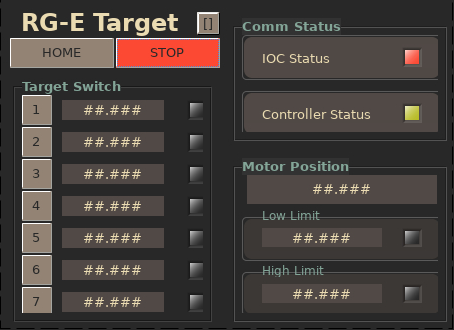
\includegraphics[]{11experiment/img/31motorx_rge.png}}
            \caption[RG-E CS-Studio main screen]{RG-E CS-Studio main screen. The HOME and A, B, C, etc buttons move the target strip to the corresponding location, the STOP button is an emergency, instant stop of the target system, and the Motor Screens button allows the user to open additional motor screens.}
            \label{fig::rge_motorx}
        \end{figure}

        In addition to this screen, other screens can be accessed through the Motor Screens menu button.
        These screens are part of the motor EPICS support module, and are left in case any debugging is necessary.
        These screens include a screen that allows for manual motor movement, a motor setup screen, a direct Command Line Interface (CLI) with the motor, and an amplifier configuration screen.
        All of these screens were developed by the Galil EPICS team \cite{farnswort2009}.

        For the user's comfort, the GUI was coloured using the Gruvbox colour palette.
        This palette is designed to keep colours easily distinguishable, contrast enough, while being pleasing for the eyes.
        Gruvbox can be found on GitHub at

        \begin{center}
            \hyperlink{https://github.com/morhetz/gruvbox}{\texttt{https://github.com/morhetz/gruvbox}}.
        \end{center}

    \paragraph{Alarm System}
        To secure the good functioning of the CLAS12 detector, all its subsystems controlled via EPICS contain PVs that specify alarm conditions.
        A centralised alarm system displays these alarms, together with their severity, associated subsystems, and pre-written guidance on how to react to them.
        For each experiment with a non-trivial target done in Hall B, the target system requires its own list of alarms.

        For the RG-E target, the set of alarms implemented and their related PVs are listed in table \ref{tab::alarmspv}.

        \begin{table}[b!]
            \caption{Alarm names, triggers, and severities for the RG-E target slow control system.}

            \begin{center}
                \begin{tabularx}{360pt}{llX}
                    \hline
                    \textbf{Name}          & \textbf{Trigger}                     & \textbf{Severity} \\
                    \hline
                    Band is not moving     & \texttt{DMC01:A\_tgttype}       =  0 & Major             \\
                    Band is moving         & \texttt{DMC01:A\_tgttype}       =  9 & Minor             \\
                    Band beyond low limit  & \texttt{DMC01:A\_tgttype}       = 10 & Major             \\
                    Band beyond high limit & \texttt{DMC01:A\_tgttype}       = 11 & Major             \\
                    Controller comm. error & \texttt{DMC01:COMMERR\_STATUS}  =  1 & Major             \\
                    IOC comm. error        & \texttt{IOC01:SR\_i\_am\_alive} =  0 & Major             \\
                    \hline
                \end{tabularx}
                \label{tab::alarmspv}
            \end{center}
        \end{table}


